
\documentclass[11pt,letterpaper]{article}
\usepackage[top=0.85in,margin=0.25in,footskip=0.75in]{geometry}


\usepackage{amsmath,amssymb}

\usepackage{float}

\usepackage{changepage}


\usepackage[utf8x]{inputenc}


\usepackage{textcomp,marvosym}


\usepackage{cite}


\usepackage{nameref,hyperref}


\usepackage[right]{lineno}


\usepackage{microtype}
\DisableLigatures[f]{encoding = *, family = * }


\usepackage[table]{xcolor}


\usepackage{array}


\newcolumntype{+}{!{\vrule width 2pt}}


\newlength\savedwidth
\newcommand\thickcline[1]{
  \noalign{\global\savedwidth\arrayrulewidth\global\arrayrulewidth 2pt}
  \cline{#1}
  \noalign{\vskip\arrayrulewidth}
  \noalign{\global\arrayrulewidth\savedwidth}
}


\newcommand\thickhline{\noalign{\global\savedwidth\arrayrulewidth\global\arrayrulewidth 2pt}%
\hline
\noalign{\global\arrayrulewidth\savedwidth}}


\raggedright
\setlength{\parindent}{0.5cm}
%\textwidth 5.25in 
\textheight 8.75in


\usepackage[aboveskip=1pt,labelfont=bf,labelsep=period,justification=raggedright,singlelinecheck=off]{caption}
\renewcommand{\figurename}{Fig}

\makeatletter
\renewcommand{\@biblabel}[1]{\quad#1.}
\makeatother




\usepackage{lastpage,fancyhdr,graphicx}
\graphicspath{ {./paperImages/} }
\usepackage{epstopdf}

\pagestyle{plain}
\fancyhf{}

\rfoot{\thepage}
\renewcommand{\headrulewidth}{0pt}
\renewcommand{\footrule}{\hrule height 2pt \vspace{2mm}}
\fancyheadoffset[L]{2.25in}
\fancyfootoffset[L]{2.25in}
\lfoot{\today}

\begin{document}
\vspace*{0.2in}

\begin{flushleft}
{\Large
\textbf\newline{Non-Local Means Denoising}
}
\newline

\\
fdmw97
\\
\bigskip

\end{flushleft}

\section*{Algorithm Description}
The Non-Local Means algorithm takes an image $v$ consiting of $I$ pixels. Then for each pixel $i \in I$ produces a new value for $i$ that is the result of a a weighted average of all the pixels in the image. This is described by the formula
$$\mathit{NL}[\mathit{u](x)} = \frac{1}{\mathit{C(x)}}\int_{\Omega}^{}\mathit{e^{-\frac{(G_{a}*|u(x+.)-u(y+.)|^{2})(0)}{h^{2}}u(y) dy}}$$
where $\mathit{x \in \Omega, C(x) = \int_{\Omega}^{}e^{-\frac{(G_{a}*|u(x+.)-u(z+.)|^{2})(0)}{h^{2}}dz}}$ is a normalizing constant\cite{paper1}
In this formula $h$ serves as an adjustable parameter to change the filtering of the image. From the above formula it can be seen that this algorithm weights the pixels in the image such that a pixel is only modified by pixels situated in gaussian neighbourhoods similar to that of $x$.
For the algorithm to be sensibly implemented the above formula must be reformulated into a discrete algorithm. Examples of these are discussed below.

\section*{Algorithm Implementations}
\paragraph{Pixelwise Implementation:}
The first discrete implementation I will be discussing is the Pixelwise Implementation. This implementation is the most faithful to the original formula given for the algorithm since it calculates the denoised value for a pixel $p$ one pixel at a time. The algorithm proposed in \cite{paper2} is as follows.
$u = (u_{1}, u_{2}, u_{3})$ is a colour image, if a pixel $p$ is selected its new value is calculated by first selecting pixels $q$ in a large search area centered on $p$, this must be bounded though to ensure an acceptable runtime. Patches of a fixed size centered around $p$ and $q$ are then compared by taking the squared Euclidean distance between them, the shorter the distance the more similar they are. This distance is then used with an exponential kernel and a normalising constant to produce the weight associated with pixel $q$. Once this has been done for all pixels in the search space around $p$ the new value for $p$ is calculated as the weighted average of the pixels $q$. After this has been repeated for all pixels $p$ in the image the new values for $p$ can be combined to form the denoised image.
\paragraph{Patchwise Implementation:}
The patchwise implementation denoises the image in patches rather than 1 pixel at a time. Its implementation according to \cite{paper2} is as follows.
The algorithm takes image $u=(u_{1},u_{2},u_{3})$ and a patch $B(p,f)$ centered around $p$ and of size $\mathit{(2f+1)\times (2f+1)}$. This patch is then compared to patches centered around pixels $q$, located in a large search area around $p$, in the same way as they are compared in the pixelwise implementation. The difference is that in the patchwise implementation the weighted average of these patch distances are used to calculate the new value of every $p$ in the patch $B(p,f)$. This saves time as less patches are compared overall.
\paragraph{Comparison:}
Pixelwise is the easier of the 2 implementations discussed in\cite{paper2} to implement. However it is less efficient as it recalculates the weight of multiple patches each time they are used for a pixel. On the other hand patchwise calculates these weights and then uses them on all the pixels in a particular patch straight away rather than having to calculate them again later.It is mentioned in\cite{paper2} that another advantage of patchwise is the higher gain in peak signal-to-noise ratio and fewer noise oscillations at edges in the image. It is worth noting that although patchwise is more efficient it offers no improvement for preserving details in the image than pixelwise\cite{paper2}. 
\section*{Effect of Paramters on Non-Local Means}
Adjusting the value of $h$ had a significant effect on the denoising of the image as can be seen below.
\begin{figure}[H]
\centering
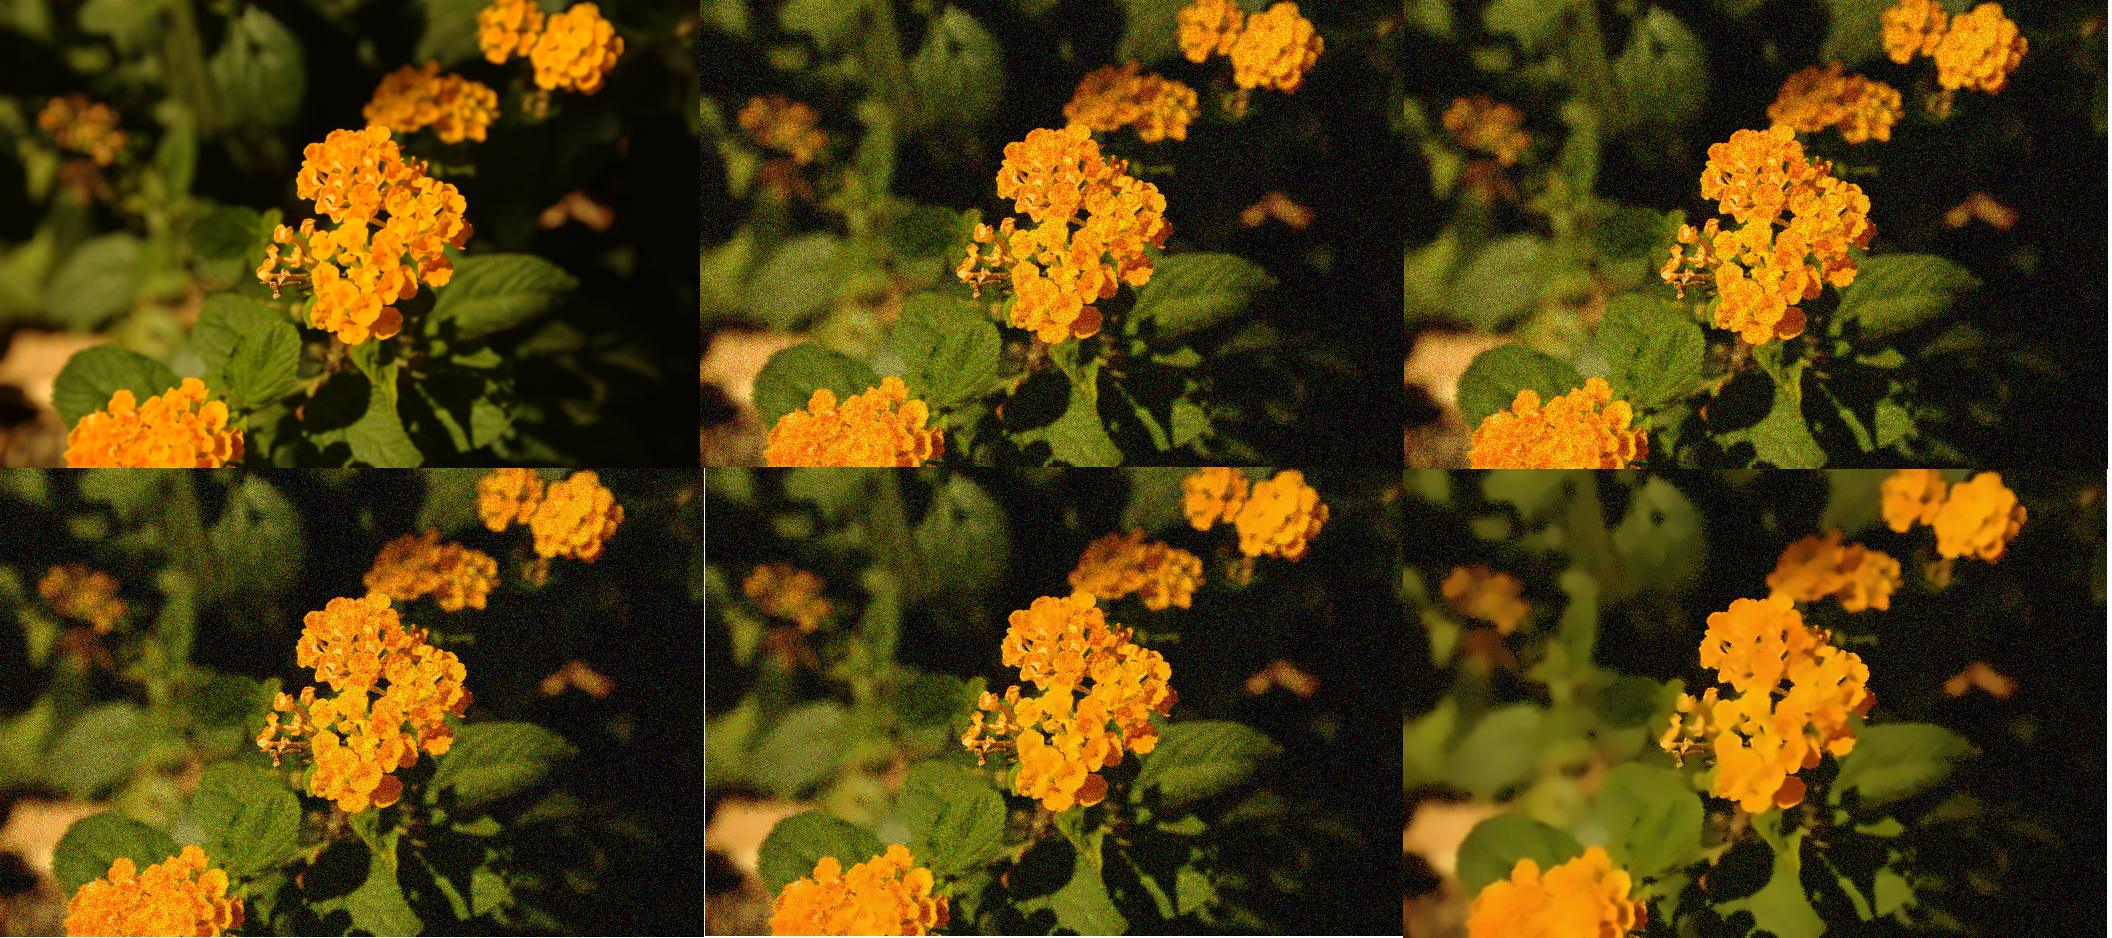
\includegraphics{combined}
\caption{Top to bottom left to right: original, noisy, h=3, h=5, h=7, h=15}
\end{figure}
As can be seen as h is increased the denoising effect becomes more pronounced. However as h grows higher more and more features and details in the image are lost as a cost to gain greater denoising.
Varying the size of the template window(tw) (size of the patch compared with the neighbourhood of $p$) reduces noise in similar parts of the image but does so at the cost of smoothing the edges between those parts of the image causing a loss in texture. This can be seen below
\begin{figure}[H]
\centering
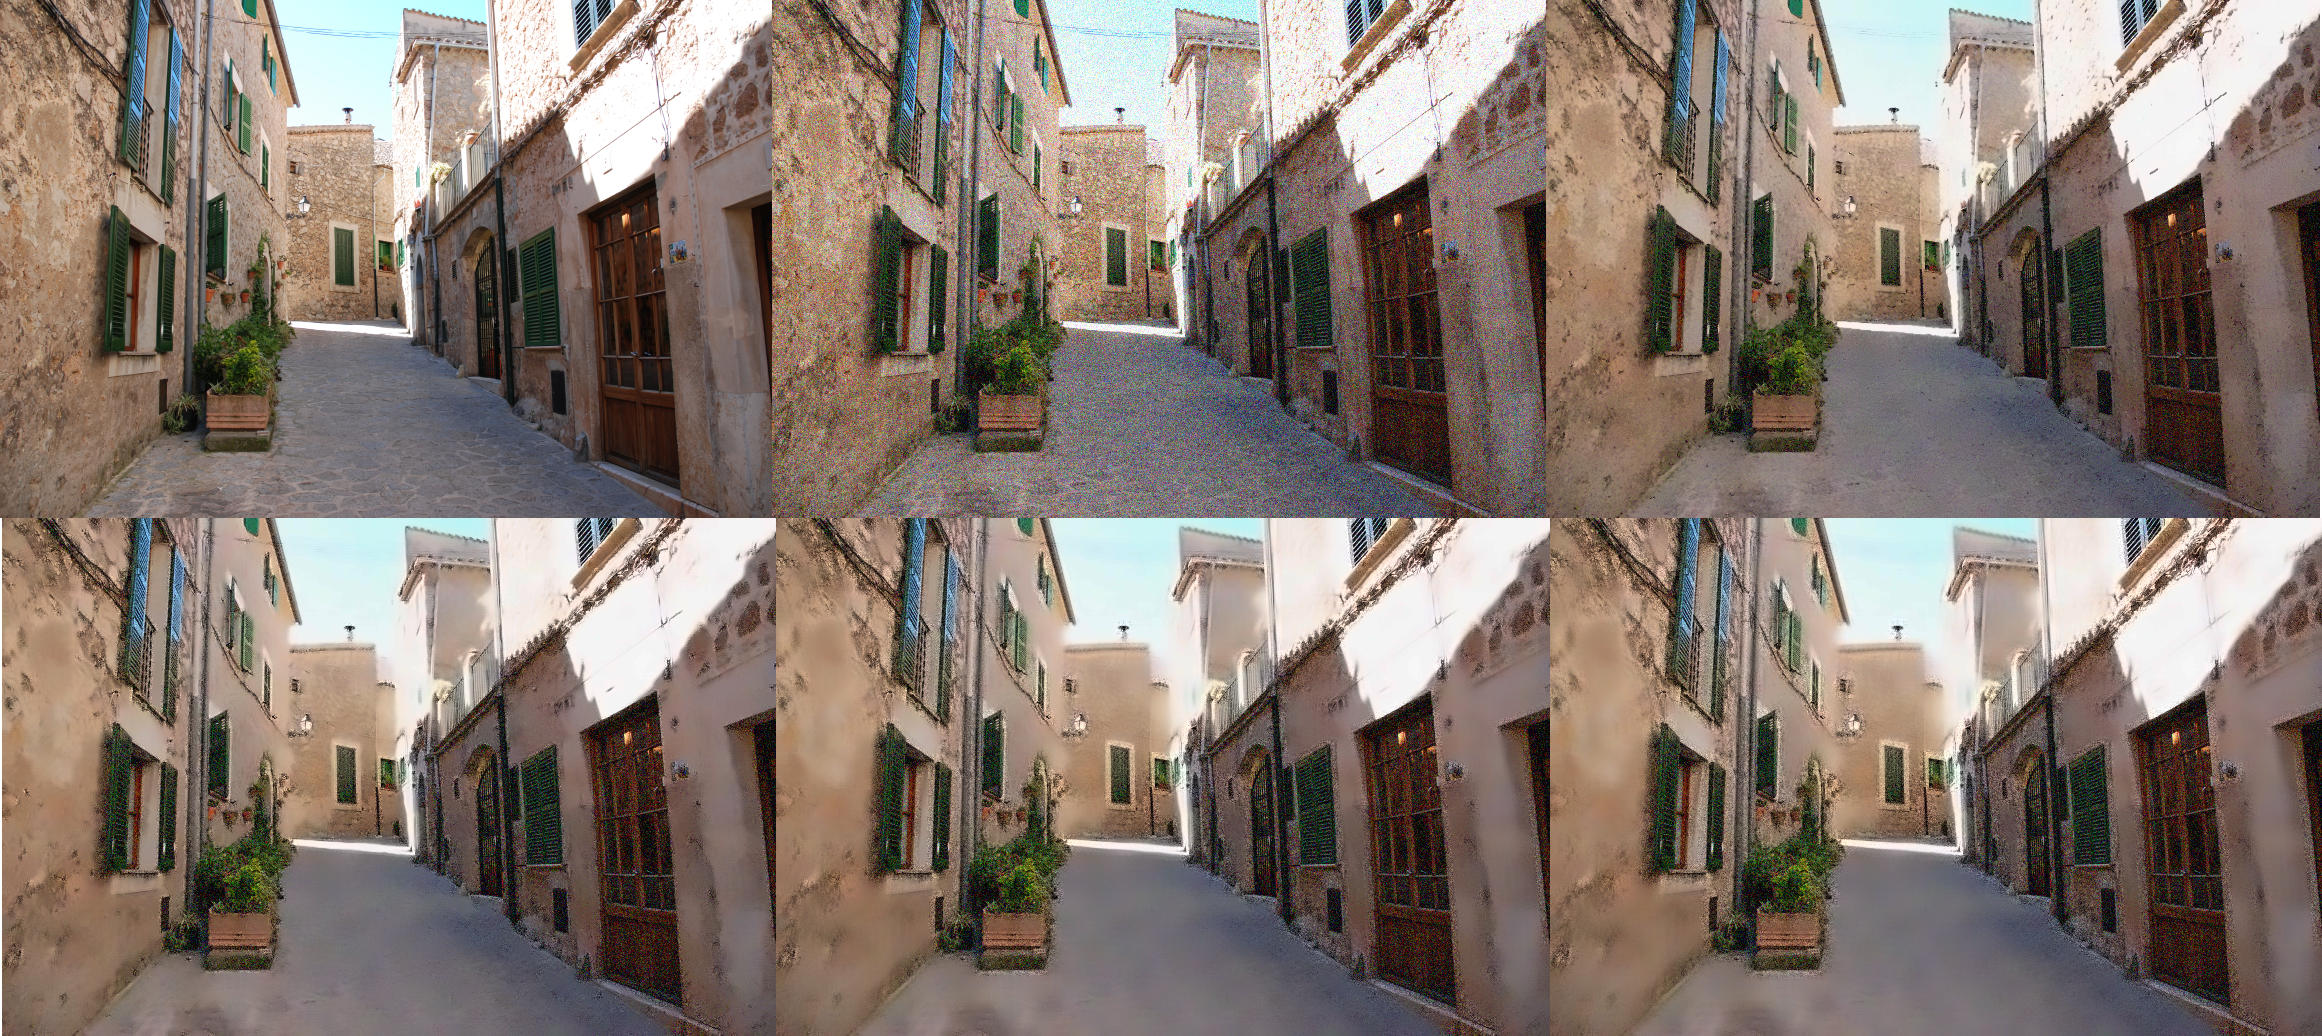
\includegraphics[height=5.9cm]{combineda}
\caption{Top to bottom left to right: original, noisy, tw=3, tw=7, tw=15, tw=21}
\end{figure}
Varying the size of the search window around $p$ had little to no effect on the result of denoising the image. With the exception of periodic images where a larger size gives much better results\cite{paper6}.

\section*{Comparison to other algorithms}
When compared to other denoising algorithms Non-local means performs very favourably. A comparison is carried out in\cite{paper3}. This comparison found that when compared to algorithms like Gaussian filter, Non-Local means maintains the structure of the original image far better keeping more details and features like hard edges.
\begin{figure}[H]
\centering
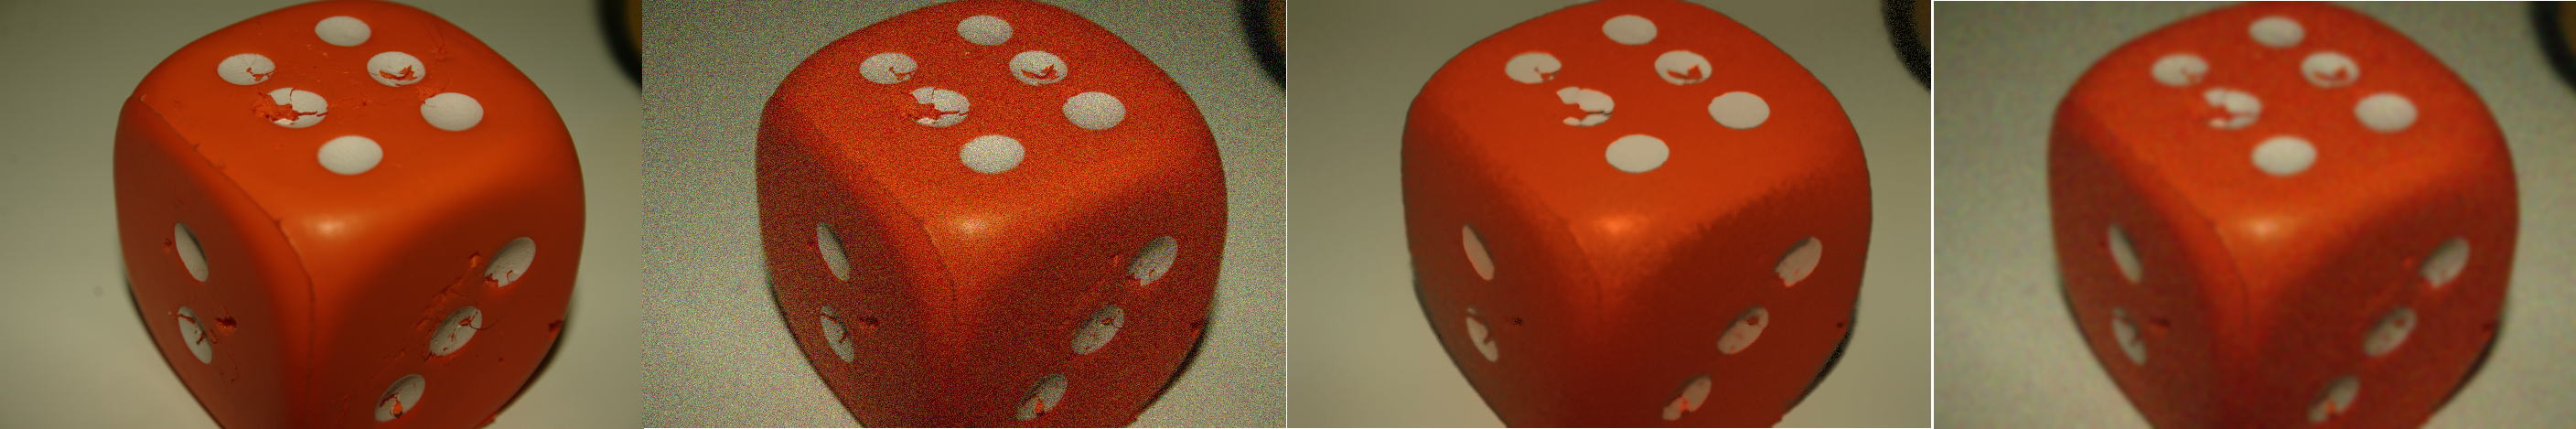
\includegraphics[width=\textwidth]{combinedd}
\caption{Left to right: original, noisy, Non-Local Means, Gaussian Filter}
\end{figure}
The above shows a blurring of edges when Gaussian filter is used instead of Non-Local means as well as worse denoising in the flat zones of the image.
The comparison\cite{paper3} also found that a major strength of Non-Local means is its ability to denoise periodic images without losing the periodic pattern. The runtime for Non-Local means is a problem compared to other algorithms for denoising as found in\cite{paper4} when it was compared to median filters. Non-Local means can also produce adhesion artefacts\cite{paper5}, this paper describes how if a pixel in a flat zone (area of similar valued pixels) is near a hard edge it will dominate the value of pixels on the other side of the edge creating an artifact. Non-Linear means tendency to over smooth textured parts of an image is also described in \cite{paper5} although this weakness can be reduced by taking an average of the denoised image and the noisy image at the end of the process to restore texture\cite{paper5}.

\section*{Extensions to Non-Local Means}
\paragraph{Gaussian Filter:}
Since the performance of Non-Local means is dependant on the variance of the noise \cite{paper7} a pre-processed image that has a lower noise variance will perform better in Non-Local means. Therefore an extension proposed in \cite{paper7} is called Enhanced-Weights NLM. This is a very simple extension to NLM and is performed by first passing the image into a Gaussian filter in order to reduce the variance of the noise. Then the image is put into NLM producing the denoised image. Downsides to this algorithm include the weaknesses of Gaussian Blur as it introduces blurring in textured regions of the image as wel as blurring at hard edges\cite{paper7}. Experimental results in the paper showed that for a variance greater than 20 EWNLM always had greater peak signal-to-noise ratio and higher perceived quality\cite{paper7}.
\paragraph{Fast Fourier Transform:}
This extension to NLM does not attempt to produce higher quality results but instead it aims to produce comparable results in less time. To do this it exploits the fact that the slowest part of NLM is calculating the Euclidean distances\cite{paper8}. This process can be replaced with a Fast Fourier Transform instead. This produces a speed increase of approximately 50 times and only a slight increase in mean squared error\cite{paper8}.
\section*{Applications of Non-Local means}
Non-Local means has many applications in medicine one such application is denoising images produced from low-dose X-ray\cite{paper9}. This is done to avoid unnecessary exposure to high amounts of radiation. Non-Local means can also be used to denoise brain segmentations\cite{paper10}. In this study it was found that a variation of NLM called ORNLM was the most effective variation of NLM as it produced denoised images that were the closest to the actual structure of the brain\cite{paper10}. NLM can also be applied to video de-interlacing. An algorithm is described in\cite{paper11} in which 2 interlaced frames are initially de-interlaced using a basic algorithm in order to first predict what the interlaced pixels should look like. Then NLM is run on the pixel being de-interlaced. This algorithm provides a distinct advantage over other de-interlacing algorithms as by using NLM it is not necessary to implement compensation for motion between the 2 frames in the algorithm as NLM removes the combing artifact that would normally be seen as a result of motion\cite{paper11}.
\begin{thebibliography}{9}
\bibitem{paper1}
Antoni Buades, and Jean-Michel Morel.
\textit{A non-local algorithm for image denoising}.
In Proceedings of the 2005 IEEE Computer Society Conference on Computer Vision and Pattern Recognition (CVPR’05) - Volume 2 - Volume 02 (CVPR ’05). IEEE Computer Society, USA, 60–65.

\bibitem{paper2}
Antoni Buades, Bartomeu Coll, and Jean-Michel Morel.
\textit{Non-Local Means Denoising}.
Image Processing Online.

\bibitem{paper3}
Antoni Buades, Bartomeu Coll, and Jean-Michel Morel.
\textit{On image denoising methods}.
CMLA Preprint.

\bibitem{paper4}
Subhojit Sarker, Shalini Chowdhury, Samanwita Laha and Debika Dey.
\textit{USE OF NON-LOCAL MEANS FILTER TO DENOISE IMAGE CORRUPTED BY SALT AND PEPPER NOISE}.
Signal \& Image Processing : An International Journal (SIPIJ) Vol.3, No.2, April 2012 .

\bibitem{paper5}
Coll, Bartomeu \& Morel, Jean-Michel.
\textit{Image and movie denoising by nonlocal means}. International Journal of Computer Vision - IJCV. 

\bibitem{paper6}
Salmon, J.
\textit{On Two Parameters for Denoising With Non-Local Means}.
IEEE Signal Processing Letters

\bibitem{paper7}
Sachin Chachada, Byung Tae Oh, Namgook Cho, San A. Phong, Daniel Manchala and C.-C.Jay Kuo.
\textit{Extension of Non-Local Means (NLM) Algorithm with
	Gaussian Filtering for Highly Noisy Images}.
2011 Visual Communications and Image Processing (VCIP), Tainan, 2011, pp. 1-4.

\bibitem{paper8}
Jin Wang, Yanwen Guo,  Yiting Ying, Yanli Liu, Qunsheng Peng.
\textit{Fast Non-Local Algorithm for Image Denoising}.
2006 International Conference on Image Processing, October 2006, pp.1429-1432

\bibitem{paper9}
Hao Zhang, Dong Zeng, Hua Zhang, Jing Wang, Zhengrong Liang, and Jianhua Ma.
\textit{Applications of nonlocal means algorithm in low-dose X-ray CT image processing and reconstruction: a review}.
Med Phys. 2017 Mar.

\bibitem{paper10}
Christian Gaser, and Pierrick Coupe
\textit{An Application of Non-Local Means Filter to Denoise Brain Segmentations}.
http://dbm.neuro.uni-jena.de/Gaser-HBM2010.pdf.

\bibitem{paper11}
Roozbeh Dehghannasiri, and Shahram Shirani.
\textit{A novel de-interlacing method based on locally-adaptive Nonlocal-means}.
2012 Conference Record of the Forty Sixth Asilomar Conference on Signals, Systems and Computers (ASILOMAR), Pacific Grove, CA, 2012, pp. 1708-1712.

\end{thebibliography}



\end{document}

